%%%% Paramétrage du TD %%%%
\def\xxactivite{ \ifprof \normalsize{TD 1 -- Corrigé } \else  \ifcolle Colle \else TD 1\fi \fi} % \normalsize \vspace{-.4cm}
\def\xxauteur{\textsl{Xavier Pessoles}}

\def\xxnumchapitre{Chapitre 2 \vspace{.2cm}}
\def\xxchapitre{\hspace{.12cm} Hyperstatisme}



\def\xxcompetences{%
\vspace{-.5cm}
\footnotesize{
\textsl{%
\textbf{Savoirs et compétences :}\\
\vspace{-.2cm}
\begin{itemize}[label=\ding{112},font=\color{ocre}] 
%\item \textit{Mod2.C34} : chaînes de solides;
\item \textit{Mod2.C34} : degré de mobilité du modèle;
\item \textit{Mod2.C34} : degré d’hyperstatisme du modèle;
\item \textit{Mod2.C34.SF1} : déterminer les conditions géométriques associées à l’hyperstatisme;
\item \textit{Mod2.C34} : résoudre le système associé à la fermeture cinématique et en déduire le degré de mobilité et d’hyperstatisme.
\end{itemize}}}}

\def\xxtitreexo{Suspension de l'AddBike}
\def\xxsourceexo{\hspace{.2cm} \footnotesize{Agrégation Sciences Industrielles de l'Ingénieur -- 2018}}


\def\xxfigures{
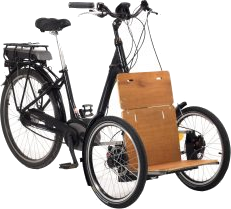
\includegraphics[width=.5\linewidth]{add_03}
}%figues de la page de garde

\input{\repRel/Style/pagegarde_TD}
\setcounter{numques}{0}
\setlength{\columnseprule}{.1pt}
\pagestyle{fancy}
\thispagestyle{plain}
\vspace{5.2cm}

\def\columnseprulecolor{\color{ocre}}
\setlength{\columnseprule}{0.4pt} 

%%%%%%%%%%%%%%%%%%%%%%%

\setcounter{exo}{0}



\begin{multicols}{2}

\subsection*{Présentation}
L'Add-Bike est un système pouvant s’adapter à tous types de vélo et doit permettre de transporter des marchandises (colis ou courses du quotidien) ou des enfants.
\begin{center}
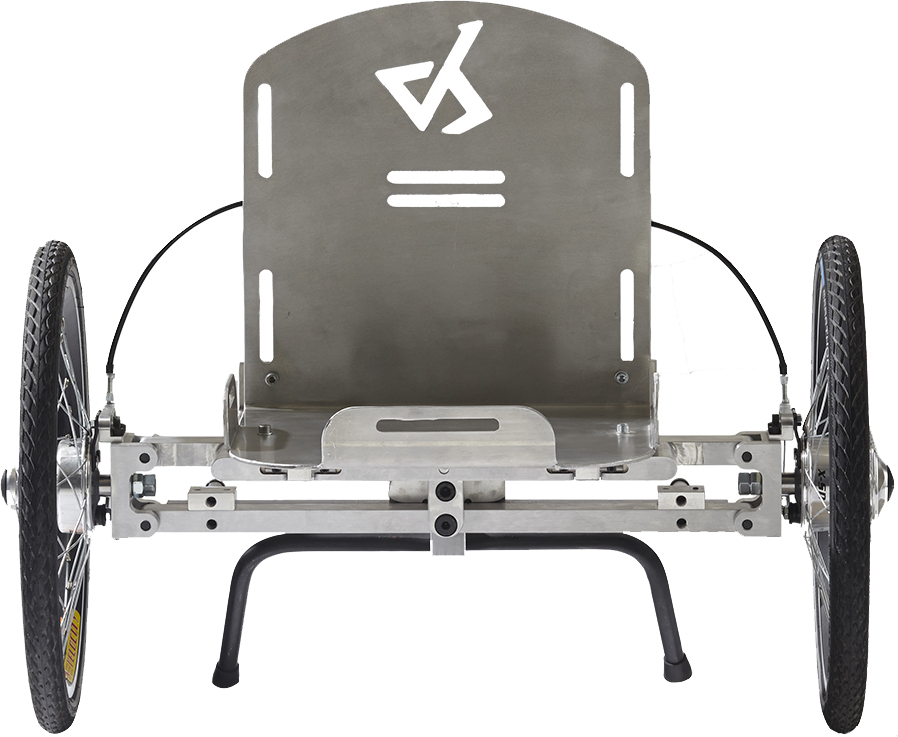
\includegraphics[width=.4\linewidth]{add_02.png}
\end{center}
Il est équipé d'un système de suspension permettant de limiter le mouvement de roulis dans les virages. 

\begin{center}
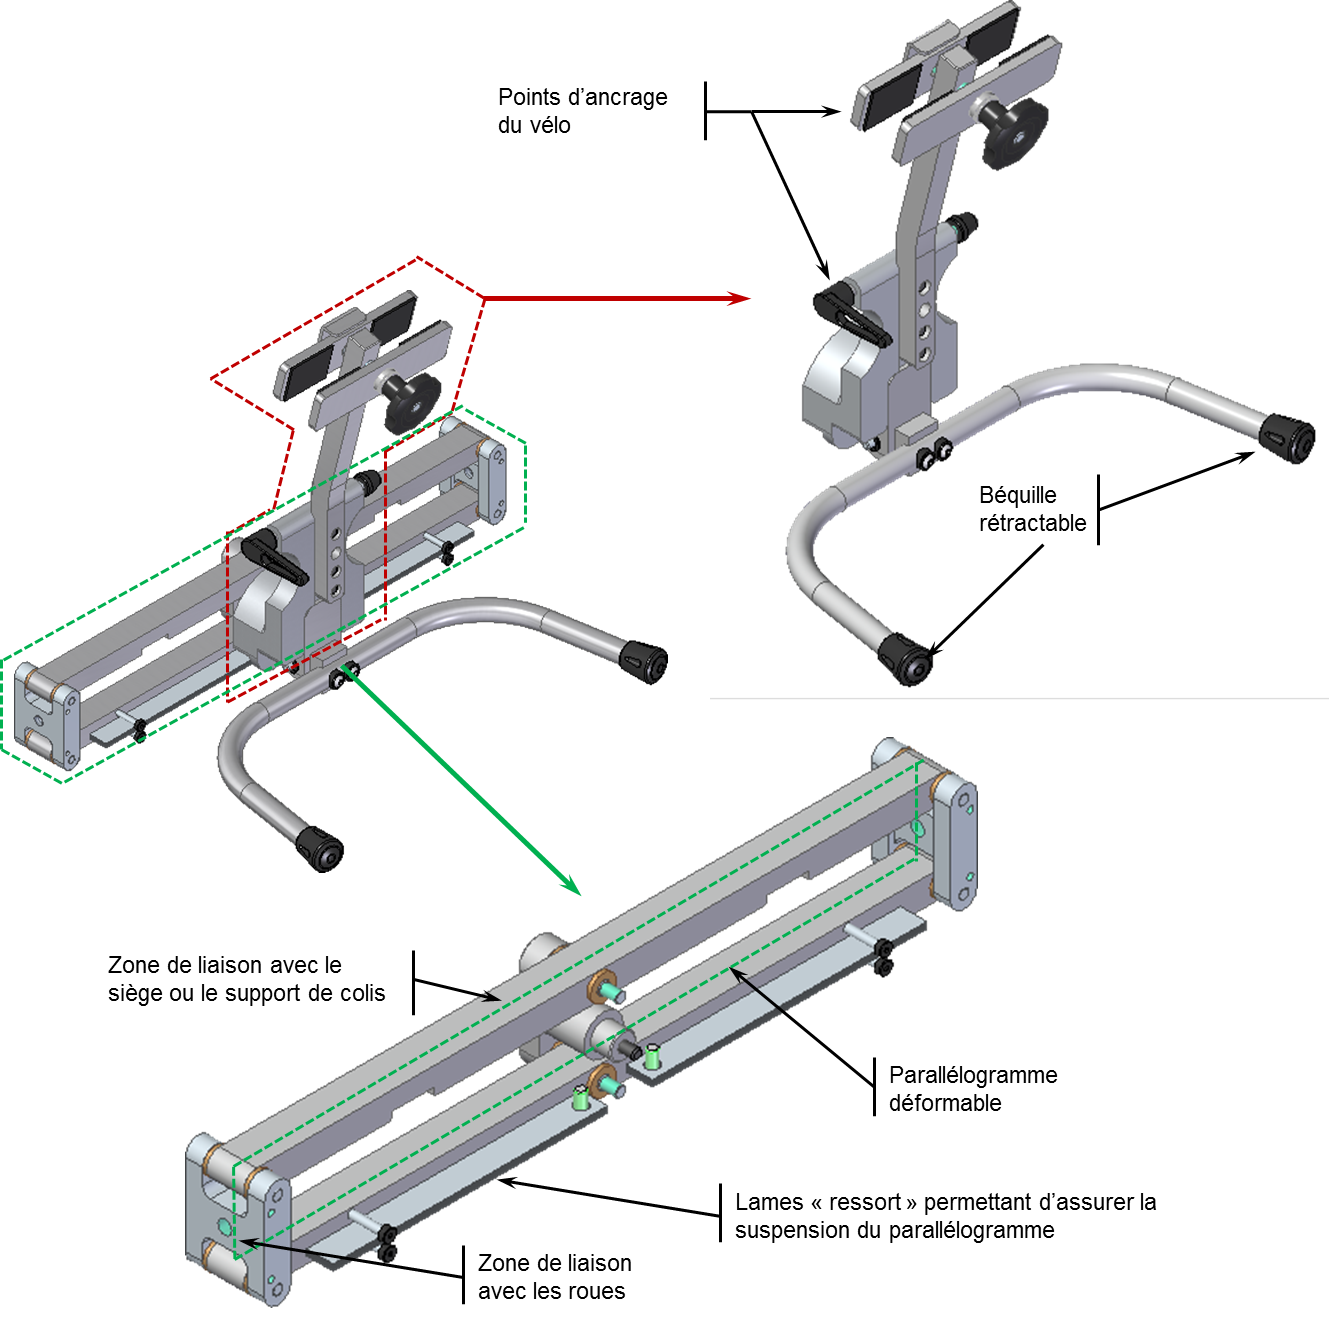
\includegraphics[width=\linewidth]{add_04.png}
\end{center}

\subsection*{Exigence 1.2 : Stabilité des occupants et des marchandises}

\begin{obj}
Pour assurer la stabilité des occupants du bi-roue, il est nécessaire de déterminer les conditions géométriques permettant de limiter l’angle de roulis (exigence 1.2.1). Ainsi, cet angle roulis ne doit pas dépasser $\beta=5\degres$  lorsque le cycliste  penche le mât vertical de $\alpha=30\degres$.
%Ces conditions géométriques devront être respectées lors de la conception de la fusée (exigence 1.2.2).
\end{obj}

\begin{center}
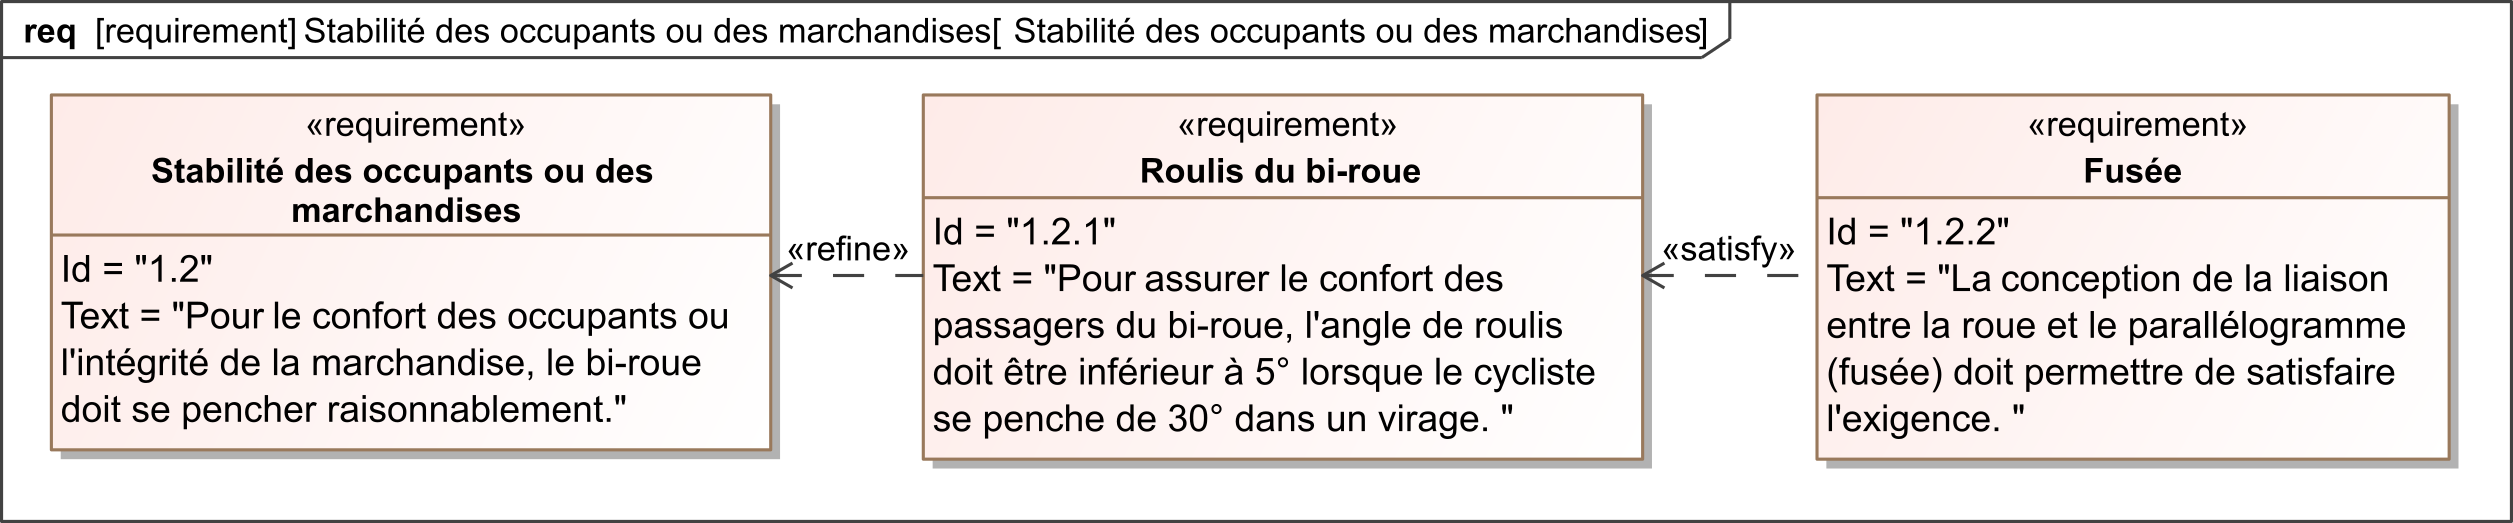
\includegraphics[width=\linewidth]{req_01.png}
\end{center}
Pour pouvoir tourner, le cycliste penche le mât vertical 04 par l’intermédiaire du guidon, ce qui conduit à la déformation du parallélogramme $ACDF$ donné dans la figure suivante et à la rotation des roues autour de l’axe horizontal longitudinal
$\vect{x_0}$. Lors de la déformation du parallélogramme, les bielles 01 et 03 ne restent pas parfaitement horizontales ; le passager assis dans le siège lié à la bielle 03, subit donc du roulis, c’est-à-dire un pivotement autour de l’axe horizontal longitudinal $\vect{x_0}$.

\begin{center}
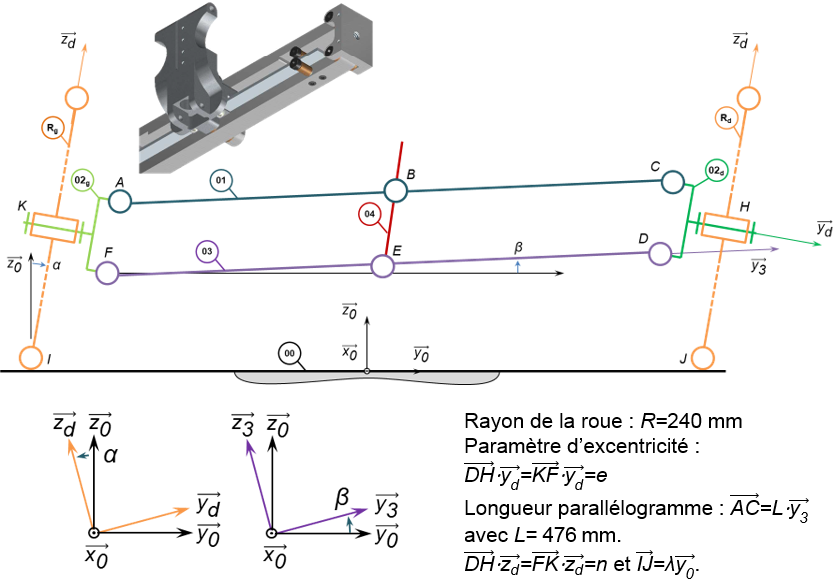
\includegraphics[width=\linewidth]{add_05.png}
\end{center}

L’angle $\beta$  correspond à l’angle de roulis des bielles 01 et 03.

\question{En réalisant une fermeture géométrique, déterminer la relation liant l’angle $\beta$  et l’excentricité $e$ des fusées 02g et 02d.}

\question{En déduire une valeur de l’excentricité $e$ permettant de valider l’exigence 1.2.1.}

\ifprof
\begin{corrige}
\end{corrige}\else\fi

\newpage

\subsection*{Exigence 1.5 : Exigences économiques -- Assemblage}
\begin{obj}
Afin de pouvoir vendre son produit à un prix attractif, la start-up doit pouvoir fabriquer et assembler son produit à un coût satisfaisant. Une maîtrise des coûts passe par la maîtrise des spécifications garantissant l’assemblage du système et par des coûts de fabrication réduits. Les objectifs sont ici de : spécifier des conditions géométriques sur les dimensions de la bielle inférieure (03) à partir des conditions de fonctionnement.
\end{obj}

\begin{center}
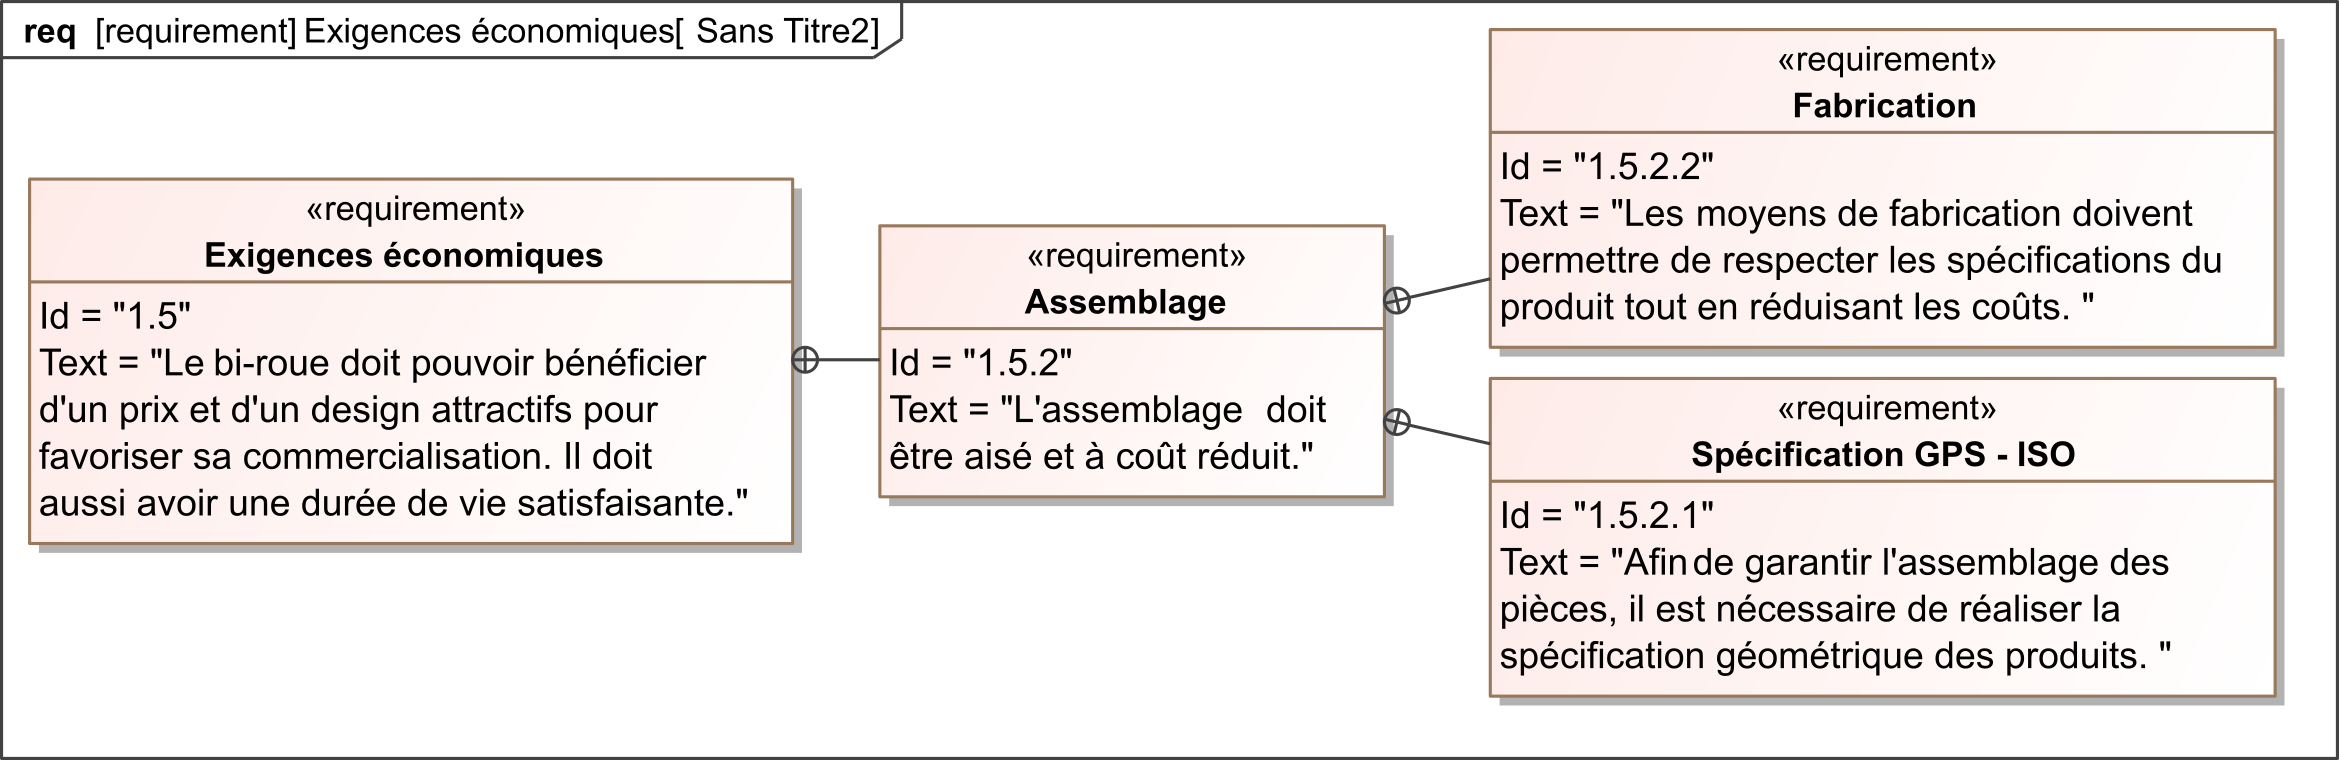
\includegraphics[width=\linewidth]{req_02.png}
\end{center}

\question{Après avoir fait un graphe de structure et sans tenir compte des roues et de leurs liaisons au sol, donner le degré d’hyperstatisme du modèle cinématique suivant.}

\ifprof
\begin{corrige}
\end{corrige}\else\fi

\begin{center}
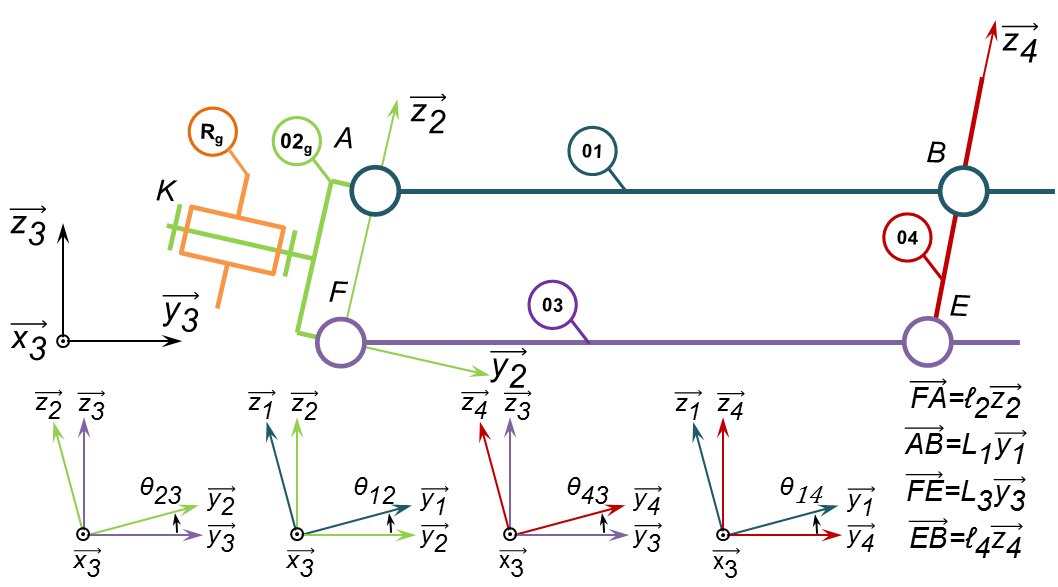
\includegraphics[width=\linewidth]{add_01.png}
\end{center}


\question{Donner les torseurs cinématiques $\torseurcin{V}{2}{3}$, $\torseurcin{V}{1}{2}$, $\torseurcin{V}{4}{3}$, $\torseurcin{V}{1}{4}$.}
\ifprof
\begin{corrige}
\end{corrige}\else\fi


\question{En utilisant une fermeture de chaîne cinématique, donner le système d’équations liant les différentes variables.}
\ifprof
\begin{corrige}
\end{corrige}\else\fi



\question{En déduire les conditions géométriques à imposer sur la bielle (03) afin de satisfaire l’assemblage du mécanisme. }
\ifprof
\begin{corrige}
\end{corrige}\else\fi



\subsection*{Synthèse}
\question{Conclure sur les méthodes qui ont permis de répondre aux exigences 1.4 et 1.5.}
\ifprof
\begin{corrige}
\end{corrige}\else\fi
\end{multicols}

